\begin{frame}[plain,containsverbatim]
	\frametitle{HE plot details: $\mat{H}$ and $\mat{E}$ matrices}
\black{Recall the data on 5 chemical elements in samples of Romano-British
pottery from 4 kiln sites:}
\begin{columns}[t]
 \begin{column}{0.55\textwidth}
\begin{CodeInput}
R> summary(Manova(pottery.mod))
\end{CodeInput}
\begin{CodeOutput}[fontsize=\footnotesize,baselinestretch=0.8]
Sum of squares and products for error:
      Al     Fe     Mg     Ca    Na
Al 48.29  7.080  0.608  0.106 0.589
Fe  7.08 10.951  0.527 -0.155 0.067
Mg  0.61  0.527 15.430  0.435 0.028
Ca  0.11 -0.155  0.435  0.051 0.010
Na  0.59  0.067  0.028  0.010 0.199
-----------------------------------
 
Term: Site 

Sum of squares and products for hypothesis:
       Al     Fe     Mg    Ca    Na
Al  175.6 -149.3 -130.8 -5.89 -5.37
Fe -149.3  134.2  117.7  4.82  5.33
Mg -130.8  117.7  103.4  4.21  4.71
Ca   -5.9    4.8    4.2  0.20  0.15
Na   -5.4    5.3    4.7  0.15  0.26
\end{CodeOutput} 
 \end{column}
 \begin{column}{0.45\textwidth}
 	\begin{itemize}
 		\item \mat{E} matrix:  Within-group (co)variation of residuals
 			\begin{itemize*}
 				\item diag:  SSE for each variable
 				\item off-diag:  $\sim$ partial correlations
 		  \end{itemize*}
 		\item \mat{H} matrix:  Between-group (co)variation of means
 			\begin{itemize*}
 				\item diag:  SSH for each variable
 				\item off-diag:  $\sim$ correlations of means
 		  \end{itemize*}
 		\item How big is \mat{H} relative to \mat{E}?
 	  \item Ellipsoids: dim(\mat{H}) = rank(\mat{H}) = $\min( p, df_h)$
  \end{itemize}
 \end{column}
\end{columns}

\end{frame}

\begin{frame}
	\frametitle{HE plot details: Scaling \H and \E}

  \begin{columns}[T]
    \begin{column}{.6\textwidth}
	  \begin{itemize}
  		\item<1-> The E ellipse is divided by $df_e = (n-p) \rightarrow$ data ellipse of
		residuals
			\begin{itemize*}
			\item<1-> Centered at grand means $\rightarrow$ show factor means in same plot.
			\end{itemize*}
		\item<1-> ``Effect size'' scaling-- $\H / df_e$ $\rightarrow$
		data ellipse of fitted values.
		\item<2-> ``Significance'' scaling-- H ellipse protrudes beyond
		E ellipse \emph{iff} $H_0$ can be rejected by Roy maximum root test
			\begin{itemize*}
			\item $H / ( \lambda_\alpha df_e )$ where $\lambda_\alpha$
			is critical value of Roy's statistic at level $\alpha$.
			\item direction of \H wrt \E \implies linear combinations that
			depart from $H_0$.
			\end{itemize*}
	  \end{itemize}
    \end{column}
    \begin{column}{.4\textwidth}
    \includegraphics<1>[width=\textwidth,clip]{figures/pottery-HE1a}
    \includegraphics<2>[width=\textwidth,clip]{figures/pottery-HE1b}
    \end{column}
  \end{columns}
\vspace{1em}  
\only<1>{
%\begin{CodeInput}
%R> heplot(pottery.mod, size="effect")
%\end{CodeInput}
\hfill\red{\textbf{\texttt{R> heplot(pottery.mod, size="effect")}}}
}	
\only<2>{
\hfill\red{\textbf{\texttt{R> heplot(pottery.mod, size="evidence")}}}
}	
\end{frame}

\begin{frame}
	\frametitle{HE plot details: Contrasts and linear hypotheses}
  \begin{columns}[T]
    \begin{column}{.6\textwidth}
	  \begin{itemize}
	    \item<1-> An overall effect \implies an \H ellipsoid of
		$s = \min( p, df_h)$ dimensions
		\item<2-> Linear hypotheses, of the form 
		$H_0 : \mat{C}_{h \times q} \, \vec{B}_{q \times p} = \mat{0}_{h \times p}$
		\implies sub-ellipsoid of dimension $h$
		\item<3-> 1D tests and contrasts \implies degenerate 1D ellipses (lines)
	  \end{itemize}
    \end{column}
    \begin{column}{.4\textwidth}
    \includegraphics<1>[width=\textwidth,clip]{figures/pottery-HE2a}
    \includegraphics<2>[width=\textwidth,clip]{figures/pottery-HE2b}
    \includegraphics<3>[width=\textwidth,clip]{figures/pottery-HE2c}
    \end{column}
  \end{columns}
\end{frame}


\begin{frame}
	\frametitle{HE plot matrices: All bivariate views}
  \begin{columns}[c]
    \begin{column}{.25\textwidth}
	  AL stands out -- opposite pattern
    \vspace{3ex}
	  $r(\widebar{Fe}, \widebar{Mg}) \approx 1$

    \end{column}
    \begin{column}{.75\textwidth}
		\begin{center}
	      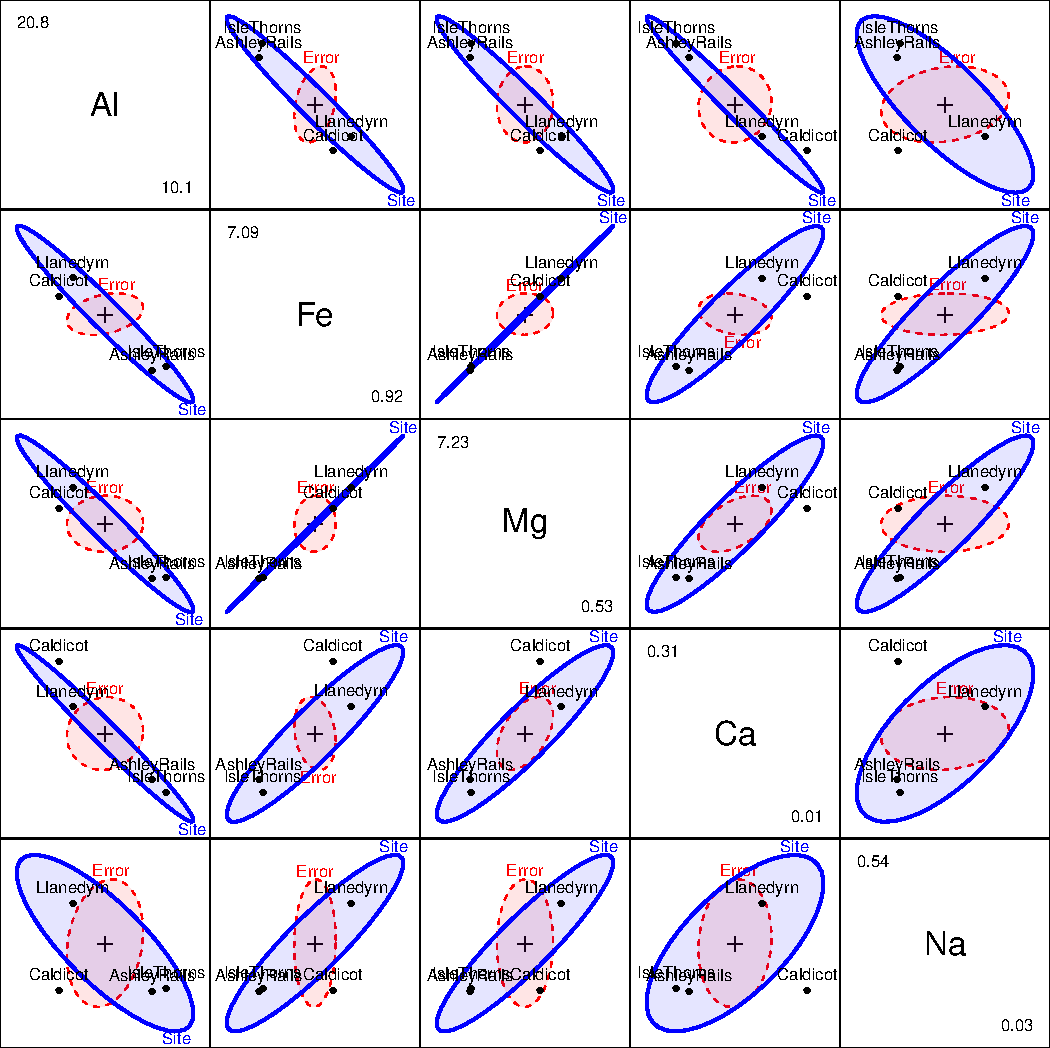
\includegraphics[height=.75\textheight,clip]{figures/pottery-HE3}
		  \\
		  \red{\textbf{\texttt{R> pairs(pottery.mod)}}}
		\end{center}
    \end{column}
  \end{columns}
\end{frame}
